%!TEX root = ../thesis.tex

\section{Introduction}
\thispagestyle{plain}


\mypar{Motivation}
  \begin{figure}[!t]
    \centering
    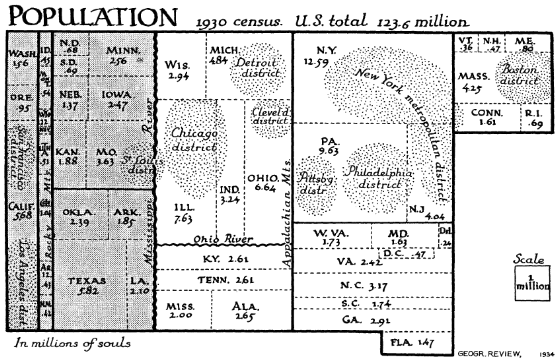
\includegraphics[scale=.5]{introduction/img/cartogram.png}
    \caption{A cartogram by Raisz~\cite{Raisz1934} made in 1934.}
    \label{fig:intro:raisz}
  \end{figure}
  In for example atlases \emph{rectangular cartograms} are used to display information, such as population or economic strength, in a spatial manner.
  In a rectangular cartogram  the geographic regions of an ordinary map are replaced by rectangles; we let these rectangles maintain adjacencies with each other to suggest geographic location and scale them proportionally to the quantities they represent.
  Raisz~\cite{Raisz1934} introduced these cartograms and provided cartograms of, for instance, land area, population (see Figure  \ref{fig:intro:raisz}) and wealth of the United States of America.
  In a rectangular cartogram it is preferable to maintain the adjacencies of the regions that are replaced by rectangles, this in order to keep the representation recognizable.
  However, this is only possible under some conditions as can be seen in Theorhem \ref{th:rect:exsitenceREctangularDual}.
  Note that the cartograms made by Raisz do not keep all adjacenies, for example, in Figure \ref{fig:intro:raisz} Florida and Alabama are not adjacent while they are in reality.

  The value of the displayed quantities, like population or wealth, often changes over time.
  When we draw a set of cartograms displaying a quantity at different moments in time, it is desirable if the adjacencies between these rectangles remain the same, no matter the moment in time.
  Moreover, it would be even better if the nature of these adjacencies, that is whether the rectangles border in a vertical or horizontal manner, does not change.
  This raises the question: When is this possible?

%  Since the size of each region will change according to the moment in time, we need to find a %rectangular cartogram that allows all area assignments.
%  \fxwarning{TODO define area addignment or change this}
%  However, even in this case it is desirable that the nature of the orientations, that is whether %it is horizontal or vertical, does not change over time.
%
%  %TODO Introduce adjeceny graph here?
%  This raises the following questions: "Which adjacency graphs can be faithfully represented by a %rectangular cartogram?" and, "Which adjacency graphs admit a cartogram that has orientations that %remain the same for all assigned areas?"
%  \fxnote{Expand on this}

\mypar{Rectangular layout}
  Mathematically, a rectangular cartogram is a  \emph{rectangular layout} (or simply \emph{layout}).
  A layout $\L$ is a partition of an axis-parallel rectangle into a finite set of interior-disjoint axis-parallel rectangles.
  A rectangular layout that has an combinatorially equivalent layout, regardless the area sizes we assign to each rectangle is \emph{area-universal}.
  \fxnote{Figure of area-universal layouts}
  The question above then becomes: For which maps can we create a area-universal layout?
  It is clear that we must leave out those maps that do not have any layouts with the same adjacencies, but this will not be enough.

\mypar{Adjacency graphs}
  We can represent the adjacencies of map regions by an \emph{adjacency graph} $G$ where each region is represented by a vertex and two vertices are connected by an edge exactly when their regions are adjacent.
  Similarly, in the \emph{adjacency graph} $\dualgraph{\L}$ of a rectangular layout $\L$ each rectangle is represented by a vertex and two vertices are connected by an edge exactly when their rectangles are adjacent.
  A layout $\L$ is a \emph{rectangular dual} of a graph $G$ if we have that $G = \dualgraph{\L}$.
  Rinsma found a graph $G$ in~\cite{Rinsma1987} that has no area-universal rectangular duals.
  That is, all rectangular layouts with $G$ as adjacency graph are not area-universal.

\mypar{One-sided layouts}
  So, unfortunately not all adjacency graphs of map regions admit area-universal duals.
  Then we would like to know which graphs do.
  For this we need to define what a one-sided layouts is.
  Note that the interior of a rectangular layout contains vertical and horizontal line segments.
  Any line segment that can not extended farther on either side is a \emph{maximal segment}.
  Such a layout is \emph{one-sided} if every maximal segment has only one rectangle on one of its sides.
  \fxnote{Figure}
  In~\cite{Eppstein2012} Eppstein et al. show that rectangular layouts are area-universal exactly when they are one-sided.
  So, Rinsma's result also implies that not all maps can be represented by an one-sided layout.


\mypar{$\mathbf{k}$-sided layouts}
  For the graphs that do not admit a one-sided, and thus area-universal, layout we still want to find layouts in which the number of adjacencies changes when areas change is as few as possible. This is beneficial for, for example, applications displaying cartograms along a continuous timescale.
  Since every time the adjacencies of the layout change, we have to compute a new rectangular layout with the right adjacencies, providing a rougher viewing experience.

  We call a layout \emph{$k$-sided} if $k$ is the smallest integer such that every maximal segment has at most $k$ rectangles on one of its sides. This is a direct generalization of one-sidedness.
  This generalization is useful because, when changing the areas of rectangles in a $k$-sided layout way more adjacencies change, in general, if $k$ is large then if $k$ is small.

  We illustrate this by comparing a typical $2$-sided and a typical $10$-sided segment.
  Let us first consider the $2$-sided segment in Figure \ref{fig:intro:2sidedBefore}, if the size of $a$ doubles only two adjacencies change, namely $dA$ and $cB$, as can been seen in Figure \ref{fig:intro:2sidedAfter}.
  While for an example of a $10$-sided segment doubling the size of a single rectangle leads to $15$ changed adjacencies, namely $aC\ aD\ bB\ bC\ bD\ bE\ cC\ cD\ cE\ cF\ dE\ dG\ eF\ eH\ fG$, as can been seen in Figure \ref{fig:intro:10sided}.

  \begin{figure}[t]
    \centering
    \begin{subfigure}[b]{0.45 \textwidth}
      \centering
      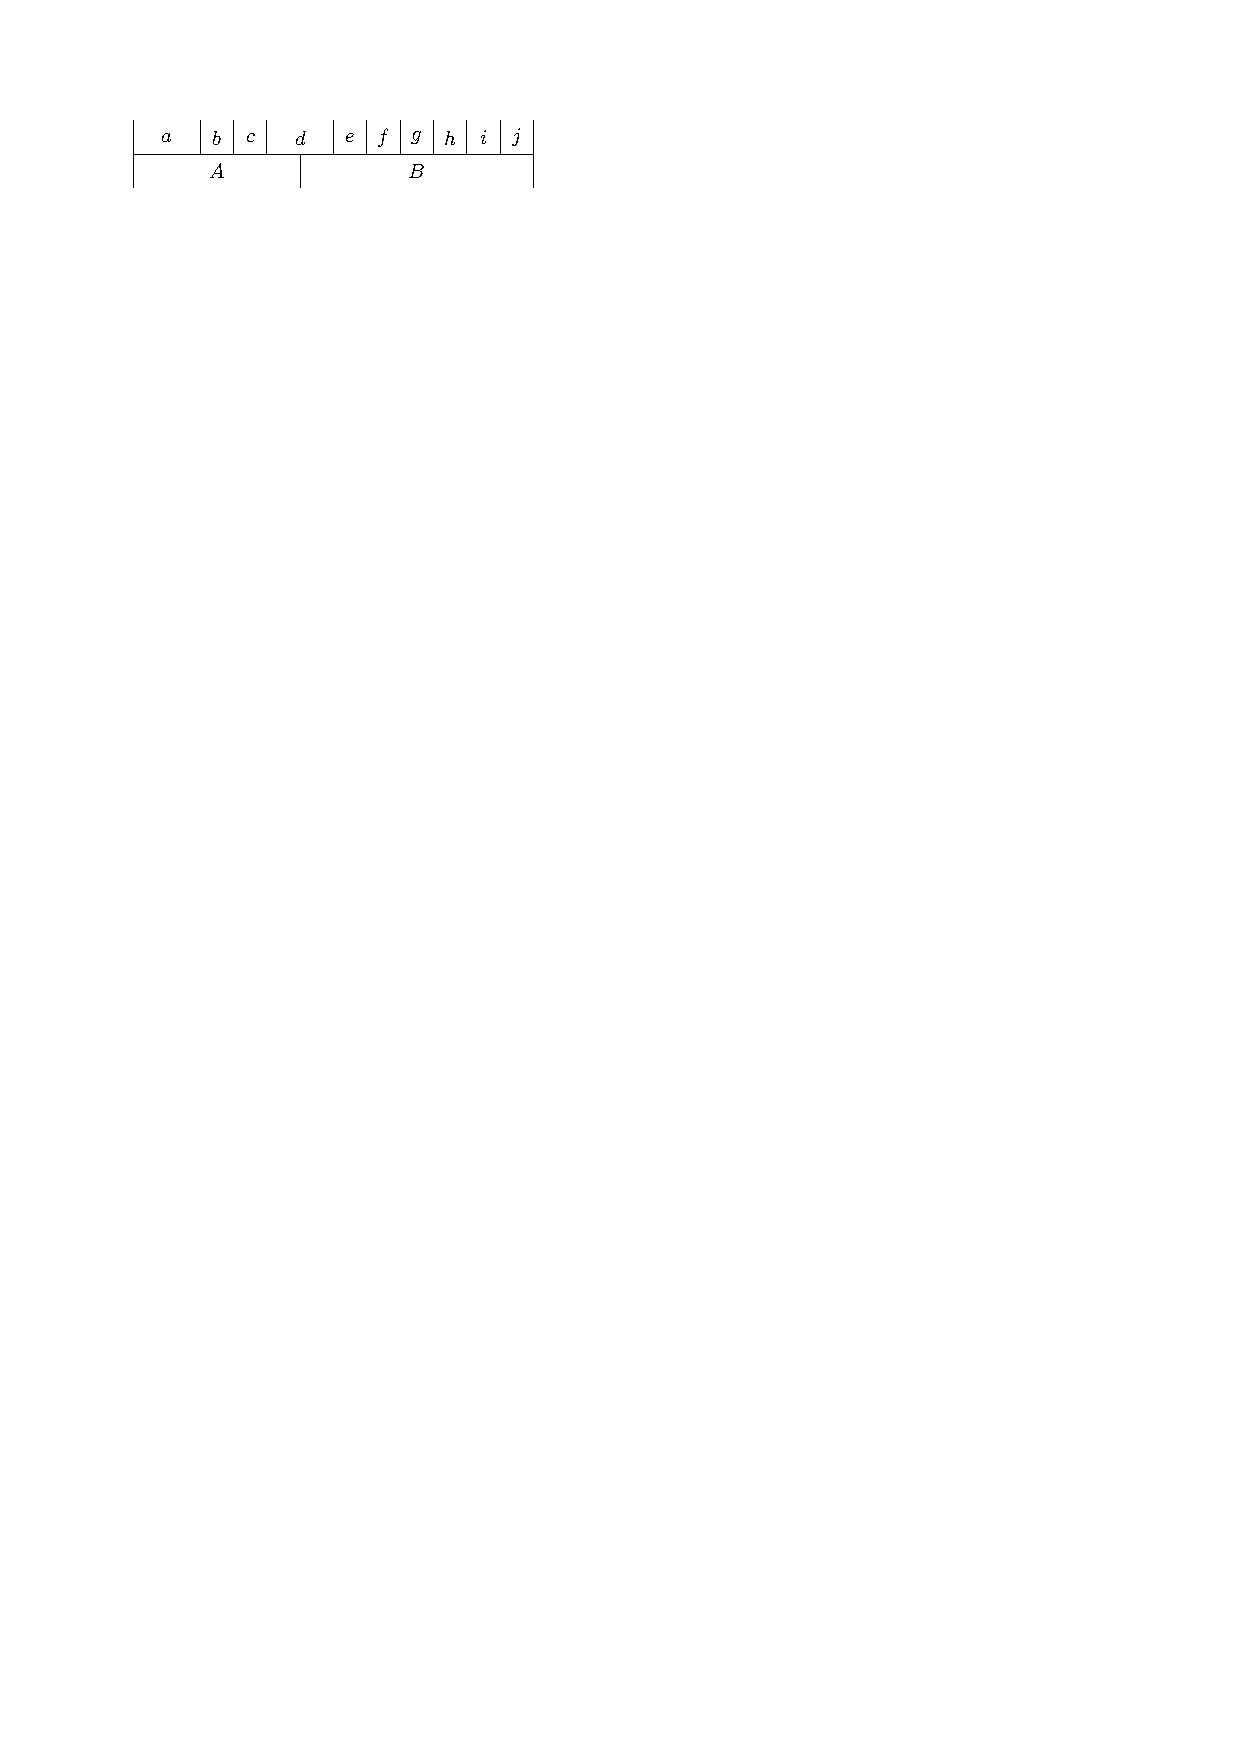
\includegraphics{introduction/img/2sidedBefore.pdf}
      \caption{Before resizing $a$}
      \label{fig:intro:2sidedBefore}
    \end{subfigure}

    \begin{subfigure}[b]{0.45 \textwidth}
      \centering
      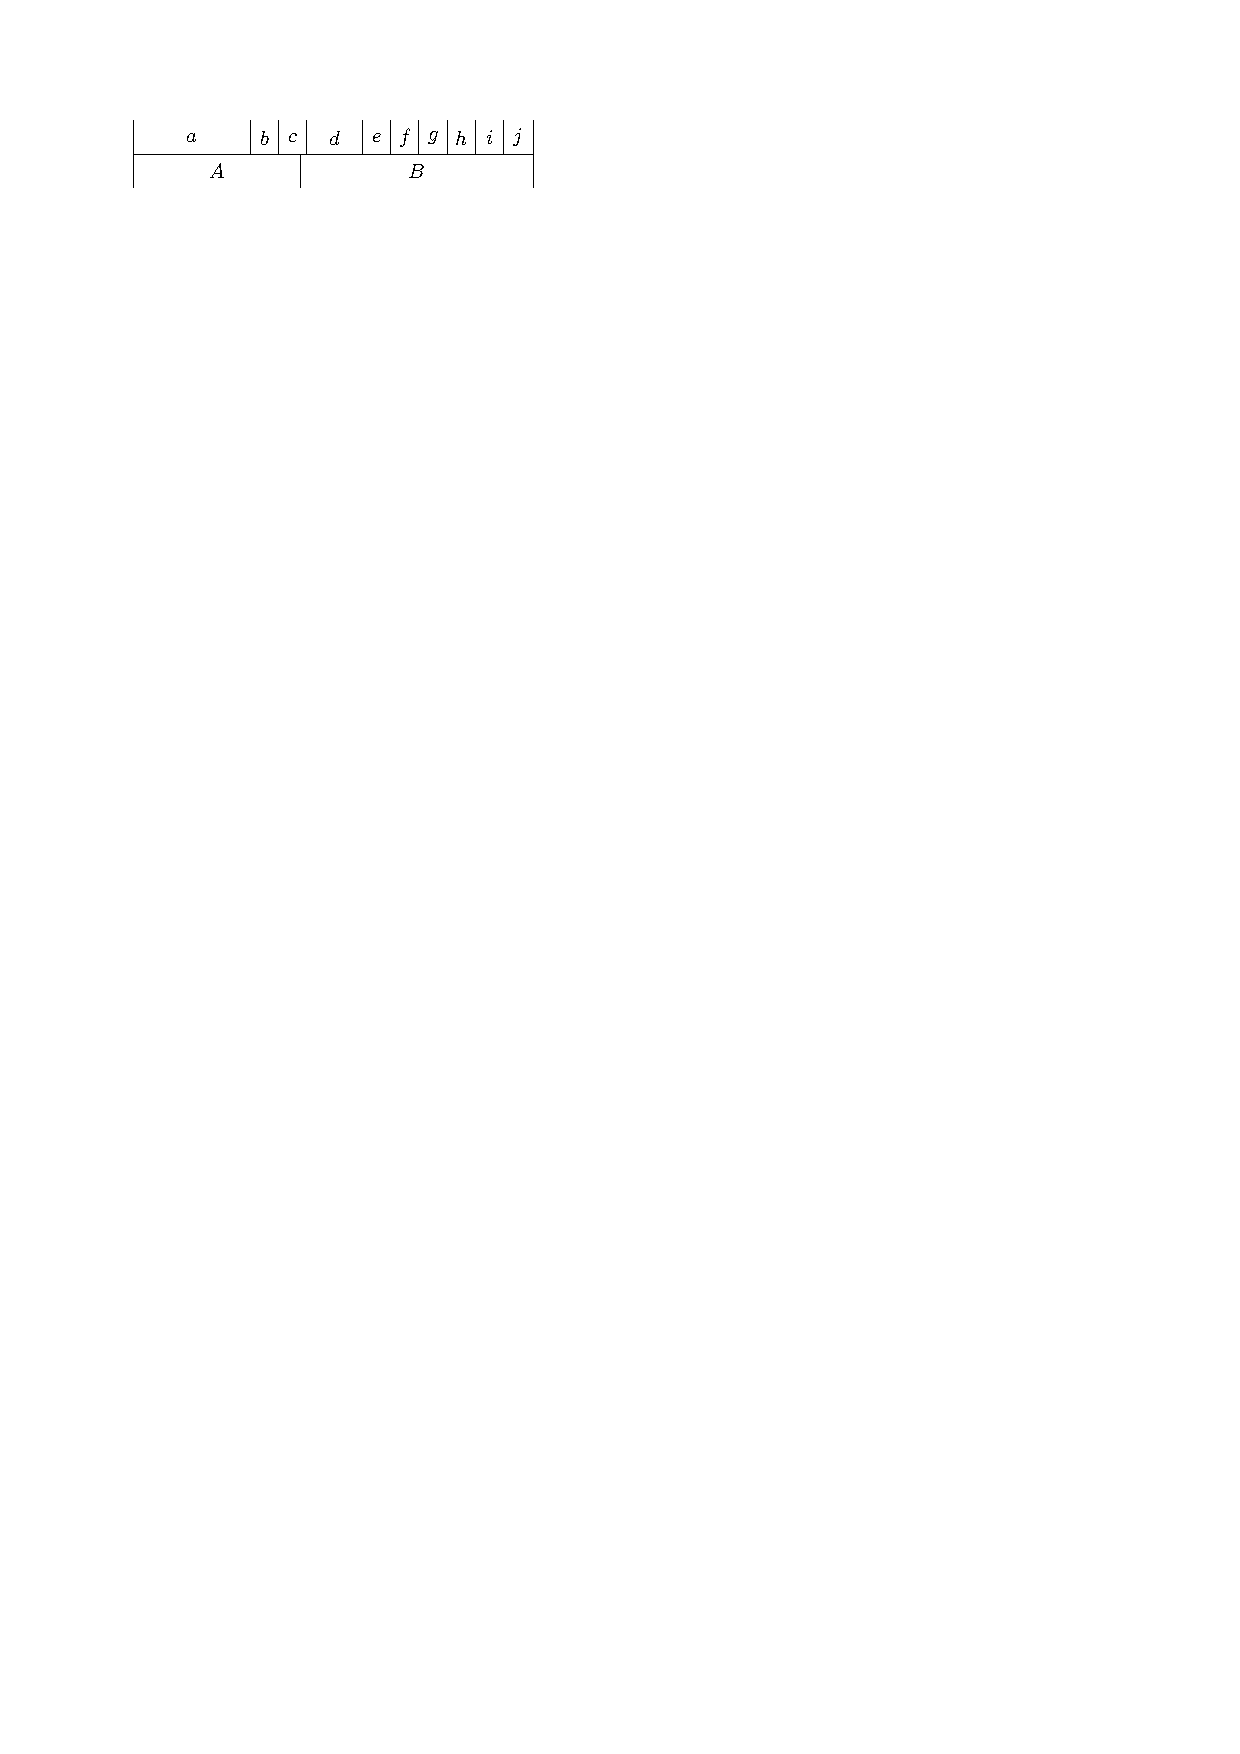
\includegraphics{introduction/img/2sidedAfter.pdf}
      \caption{After resizing $a$}
      \label{fig:intro:2sidedAfter}
    \end{subfigure}
    \caption{A 2-sided segment}
    \label{fig:intor:2sided}
  \end{figure}

  \begin{figure}[b]
    \centering
    \begin{subfigure}[b]{0.45 \textwidth}
      \centering
      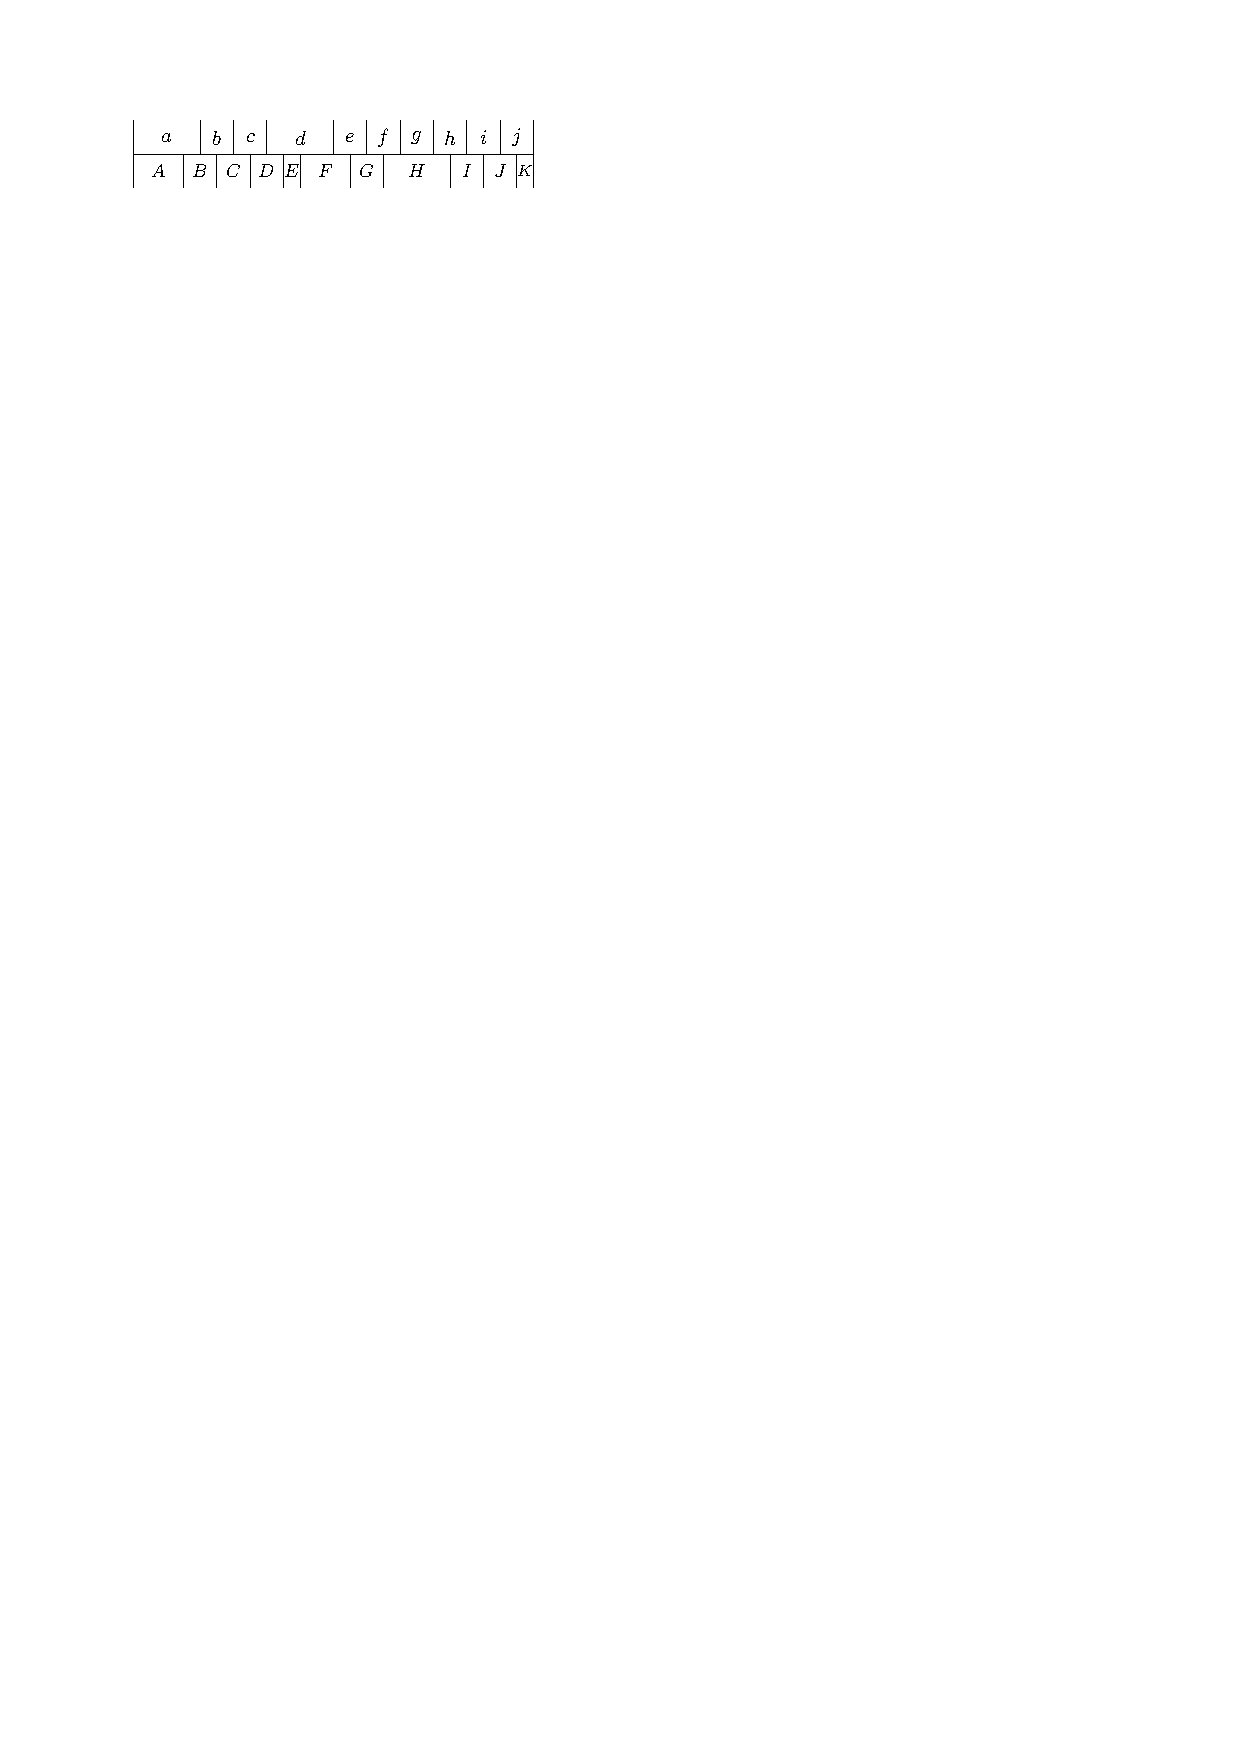
\includegraphics{introduction/img/10sidedBefore.pdf}
      \caption{Before resizing $a$}
      \label{fig:intro:10sidedBefore}
    \end{subfigure}

    \begin{subfigure}[b]{0.45 \textwidth}
      \centering
      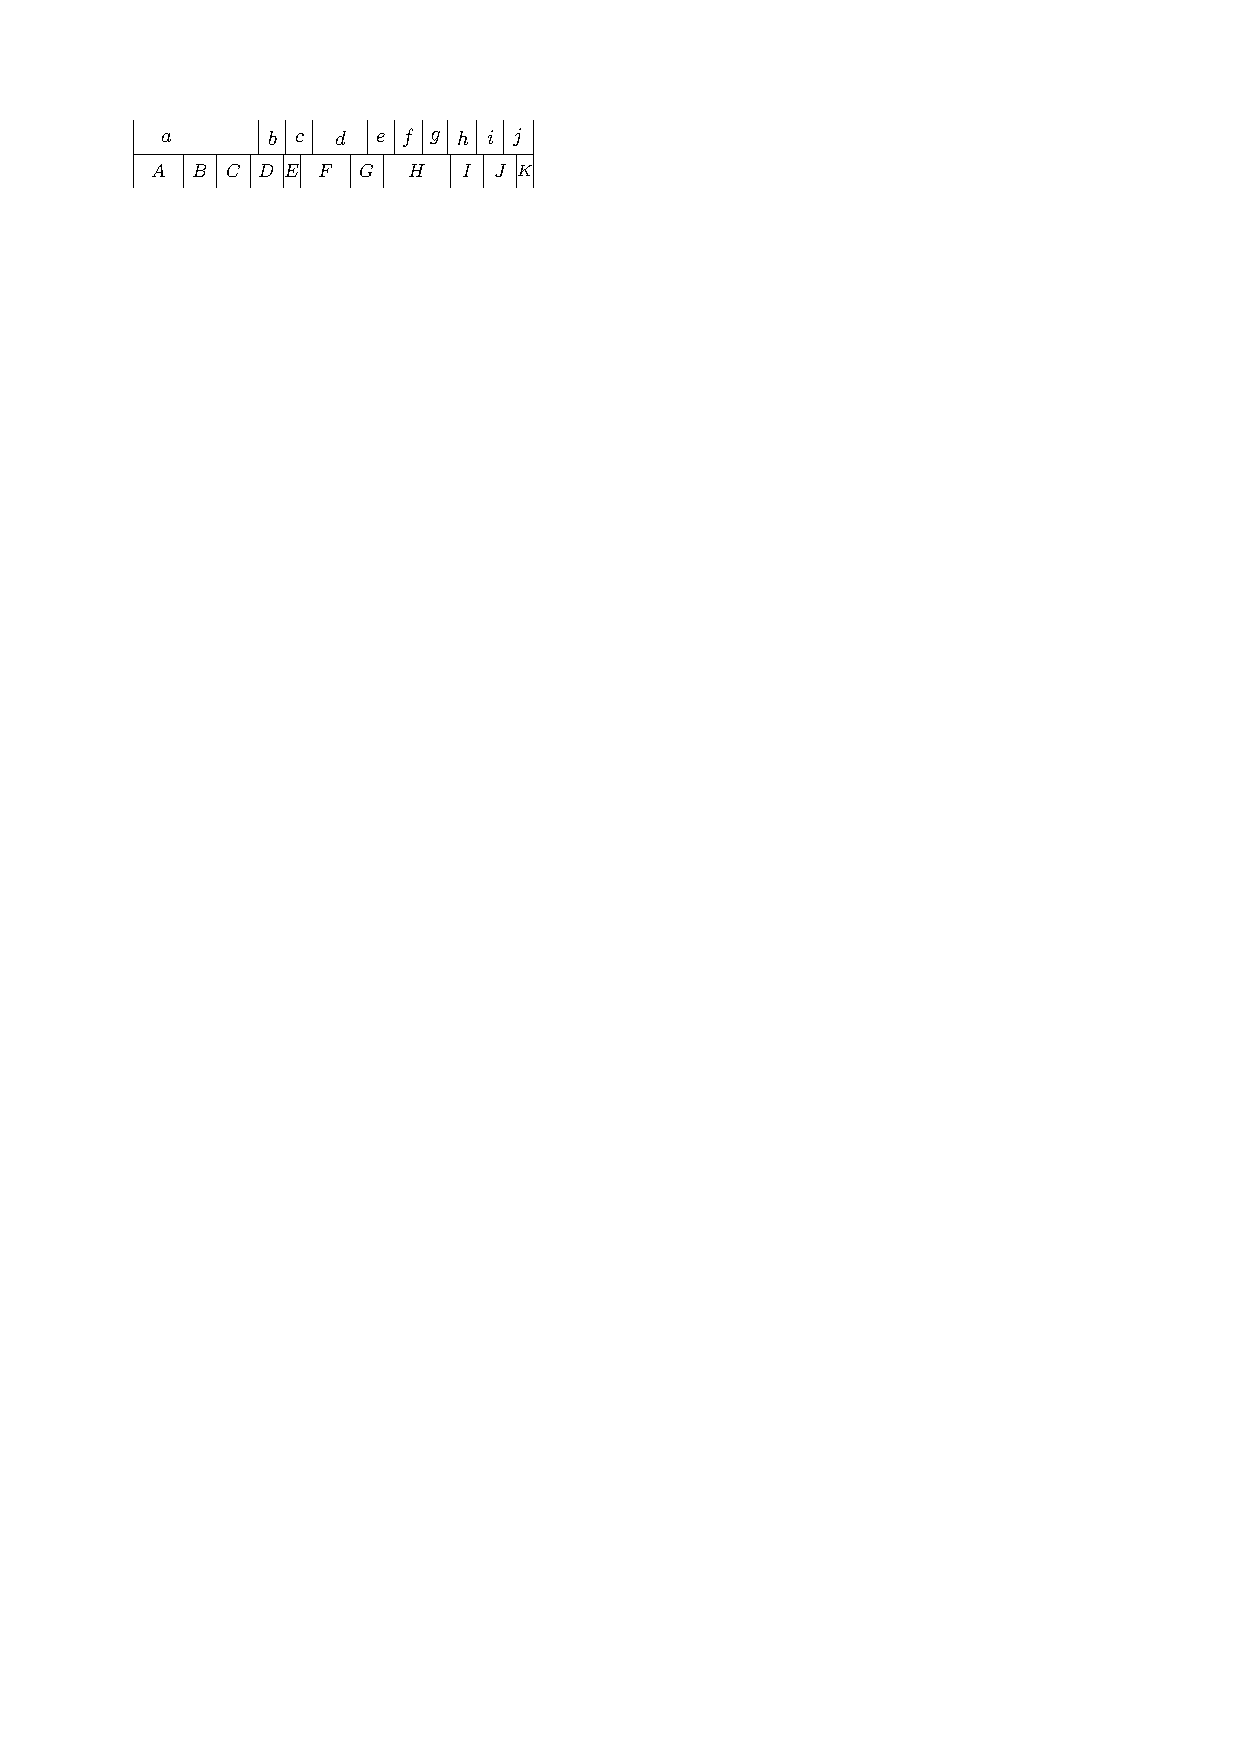
\includegraphics{introduction/img/10sidedAfter.pdf}
      \caption{After resizing $a$}
      \label{fig:intro:10sidedAfter}
    \end{subfigure}
    \caption{A 10-sided segment}
    \label{fig:intro:10sided}
  \end{figure}


\mypar{Results}
  In this thesis we provide two results on $k$-sidedness.
  \begin{enumerate}
    \item There is a family of graphs $G_k$ that for any $k \in \N$ has members that are not $k$-sided (Theorem \ref{fix:th:family}).
    \item Triangulations of the $k$-gon $G$ that have a corner assignment without separating 4-cycles are $d-1$-sided, where $d$ is the maximal degree of the vertices of $G$. (Theorem \ref{th:dsided})
  \end{enumerate}

  \fxnote{Context}


\mypar{Combinatorially equivalent}
  We say two layouts are  \emph{combinatorially equivalent} or simply \emph{equivalent} when their rectangles have the same adjacencies with the same orientation(horizontal or vertical) between their rectangles. \fxwarning{Look at definition by speckmann}

  Consider for example Figure \ref{fig:intr:segmentdefs}, the three highlighted lines are all line segments. However, only the red and blue segment are maximal segments. The red segment is one-sided and the blue segment is $2$-sided and the whole layout is $2$-sided. Furthermore, the layout in Figure \ref{fig:intr:vertonesided} is $4$-sided.

  \begin{figure}[b]
      \centering
      \begin{subfigure}[b]{0.45 \textwidth}
        \centering
        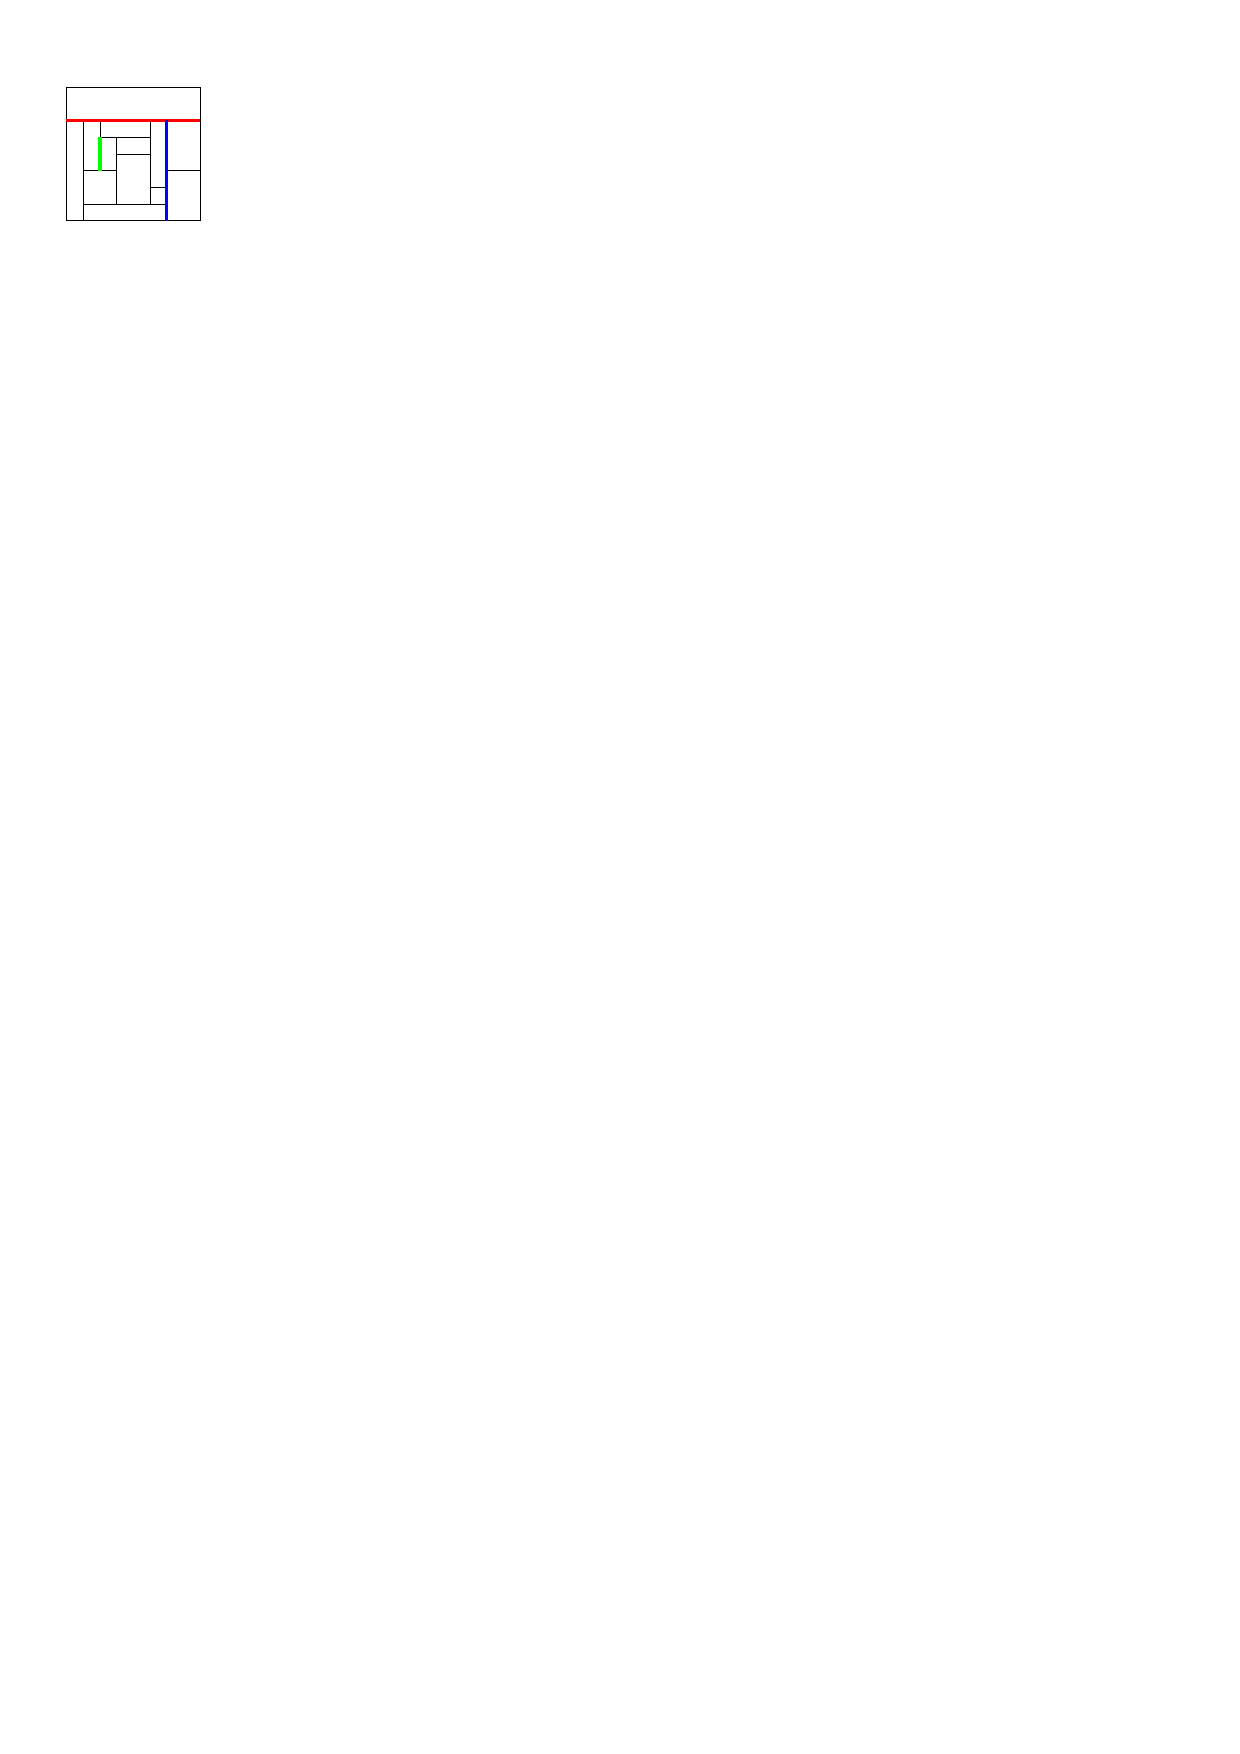
\includegraphics[scale=1]{rectangularDuals/img/segmentdefs}
        \caption{A rectangular layout.}
        \label{fig:intr:segmentdefs}
      \end{subfigure}
      ~
      \begin{subfigure}[b]{0.45 \textwidth}
        \centering
        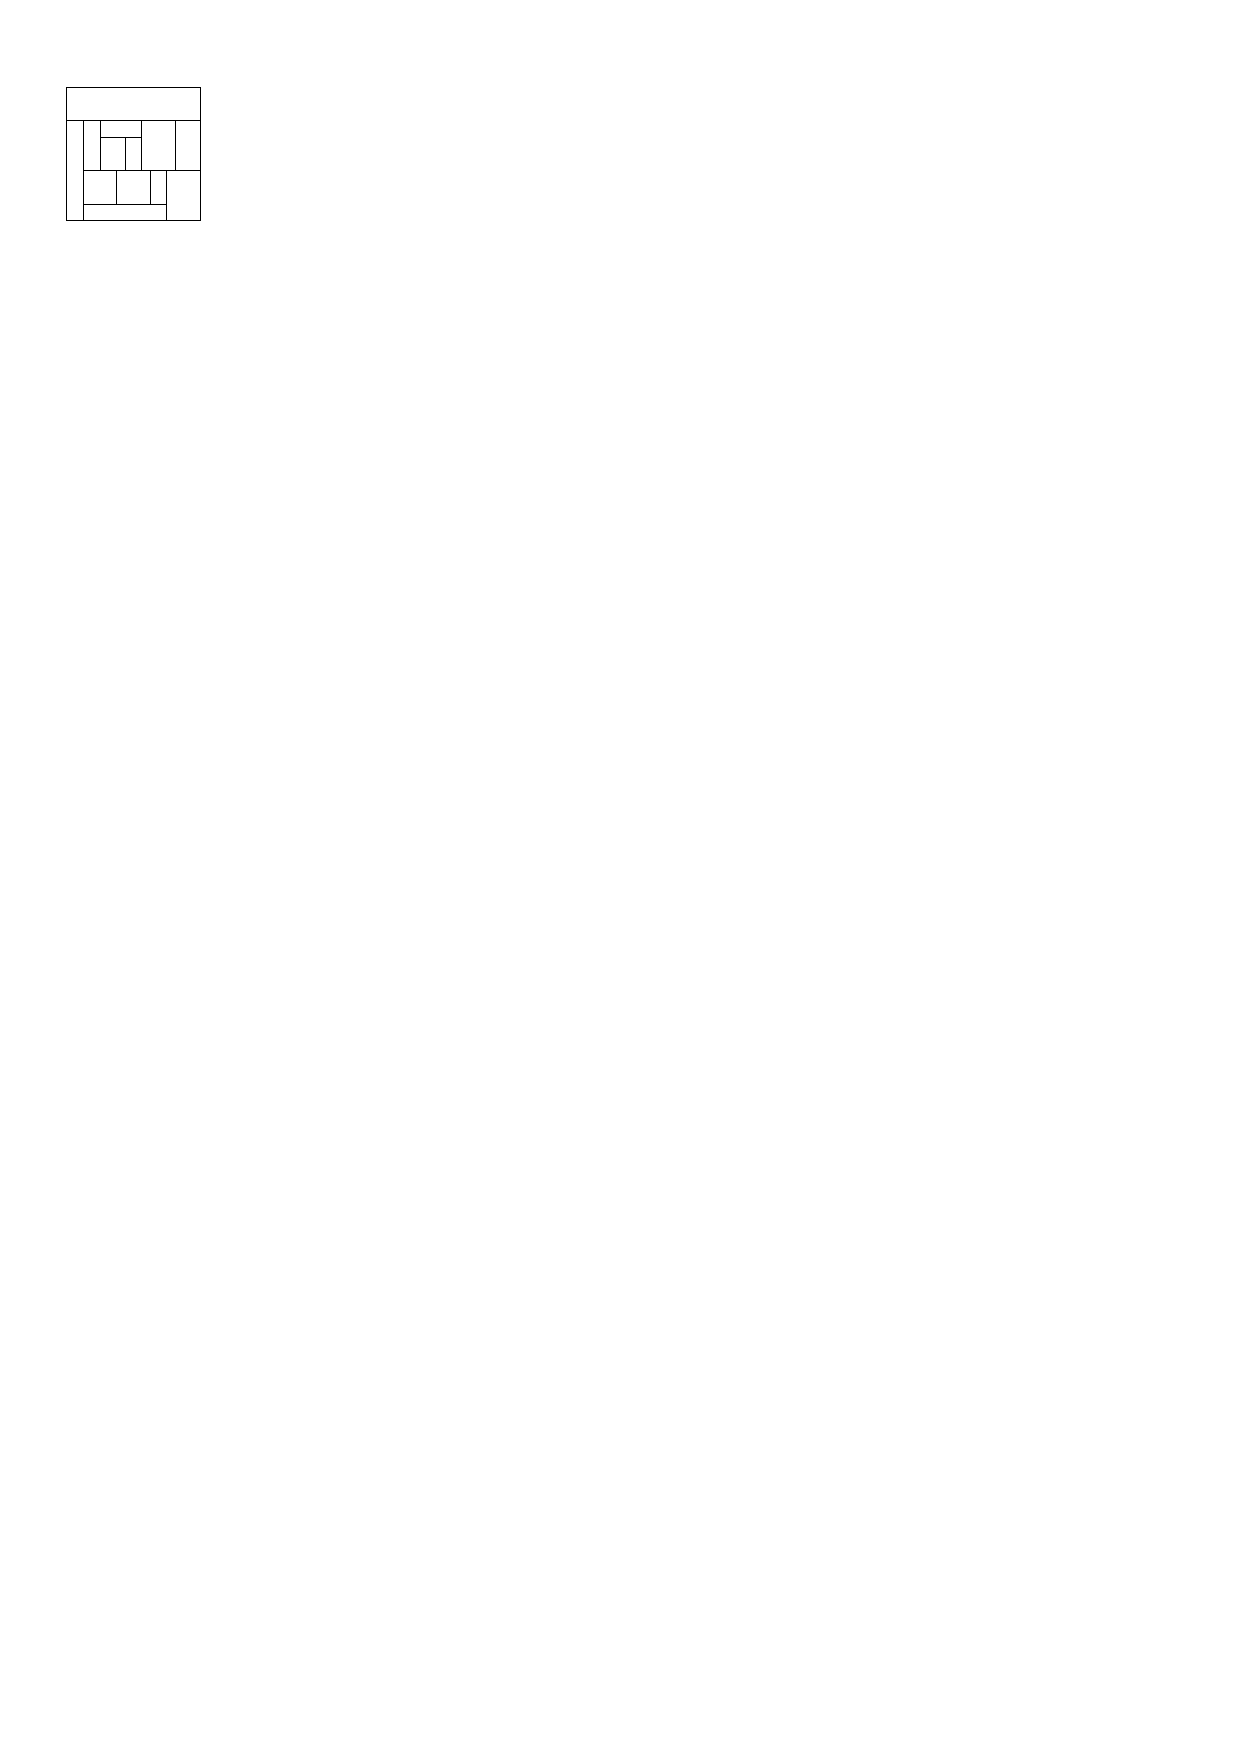
\includegraphics[scale=1]{rectangularDuals/img/vertonesided}
        \caption{Another rectangular layout.}
        \label{fig:intr:vertonesided}
      \end{subfigure}
      \caption{Rectangular layouts}
      \label{fig:intr:graphs}
  \end{figure}

\mypar{Graphs}
  A \emph{graph} $G$ is an abstraction of a network. The objects are represented by a set of \emph{vertices}.
  Connections between objects are represented by a set of \emph{edges}; each edge connects two vertices.
  Two distinct edges do not have the same vertices and no edge starts and ends at the same vertex.
  That is, graphs in this thesis are \emph{simple}. An edge is \emph{incident} to a vertex $v$ if that edge connects $v$ to another vertex.
  The \emph{degree} of a vertex is the number of edges incident to this vertex.
  All graphs in this thesis are \emph{planar}.
  That is, they can be embedded in the plane without their edges crossing. A \emph{face} is connected component of the maximal subset of the plane that is disjoint from the embedded graph. The \emph{degree} of a face is the number of vertices on its boundary.
  A face of degree $3$ is a \emph{triangular} face. The \emph{outer face} is the one and only unbounded face.
  A vertex is \emph{incident} to a face when it lies on its boundary.

  All graphs in this thesis are \emph{triangulations of the $k$-gon}. A triangulation of the $k$-gon has an outer face of degree $k$ and interior faces of degree $3$.
  Vertices bordering the outer face are \emph{outer vertices} while all other vertices are \emph{interior vertices}.
  Triangulations of the $k$-gon are called \emph{(plane) triangulated graphs} by some other authors.

\mypar{Rectangular duals}
  Two vertices are \emph{adjacent} when they are connected by an edge. Two rectangles are \emph{adjacent} when their boundaries overlap. A \emph{rectangular dual} of $G$ is a rectangular layout whose adjacencies are the same as those of $G$ for a bijection between vertices and rectangles.

\mypar{Corner assignments}
  If we want to determine which graphs do have a rectangular dual, then we need to introduce the notion of a \emph{corner assignment}.
  A corner assignment $\ext G$ of $G$ is an augmentation of $G$ with $4$ vertices (which we call its \emph{poles}), such that every interior face has degree $3$, the exterior face has degree $4$ and all poles are incident to the outer face.

  \fxwarning{Take definition from paper}
  A corner assignment of $G$ only exists if $G$ is a triangulation of the $k$-gon for some $k$. Otherwise, there is no way of adding poles that makes all the interior faces of degree $3$. Because of this, we only consider triangulations of the $k$-gon in this thesis. A corner assignment $\ext G$ of $G$ is an example of a triangulation of the $4$-gon. Each corner assignment fixes which rectangles are in the corners of the rectangular dual $\L$, which explains the terminology.

\mypar{Existence and uniqueness}
  Now we can state which graphs admit a rectangular dual. The following result was shown independently by Kozminski and Kinnen \cite{Kozminski1984} and Ungar \cite{Ungar1953}.

  \begin{thrm}[Existence of a rectangular dual]
    \label{th:rect:exsitenceREctangularDual}
    A triangulation of the $k$-gon $\G$ has a rectangular dual if and only if it has a corner assignment without separating triangles $\ext \G$.
  \end{thrm}

  A graph $G$ can have multiple rectangular duals. $G$ can even have duals that are not equivalent. An example is given by the two non-equivalent duals of the same graph given in Figure \ref{fig:intr:graphs}.
  \fxwarning{Add wrapfig this other figure is too big}

\mypar{Rectangular cartograms}
  A rectangular cartogram is the rectangular dual of the adjacency graph of the map $G$.
  If the areas change it might be that a certain rectangular layout can not fulfill its adjacencies anymore and we have to switch to another non-equivalent rectangular dual of $G$.

  We would like to find a rectangular dual that has adjacencies that hold regardless of the area sizes we assign to each rectangle. We say such a dual is \emph{area-universal}.
  Eppstein et al. have shown that rectangular duals are area-universal exactly when they are one-sided.~\cite{Eppstein2012} Unfortunately not all graphs admit a one-sided dual. One such graph, displayed in Figure \ref{fig:intro:rinsma},  is given by Rinsma.~\cite{Rinsma1987}

  \begin{figure}[!t]
    \centering
    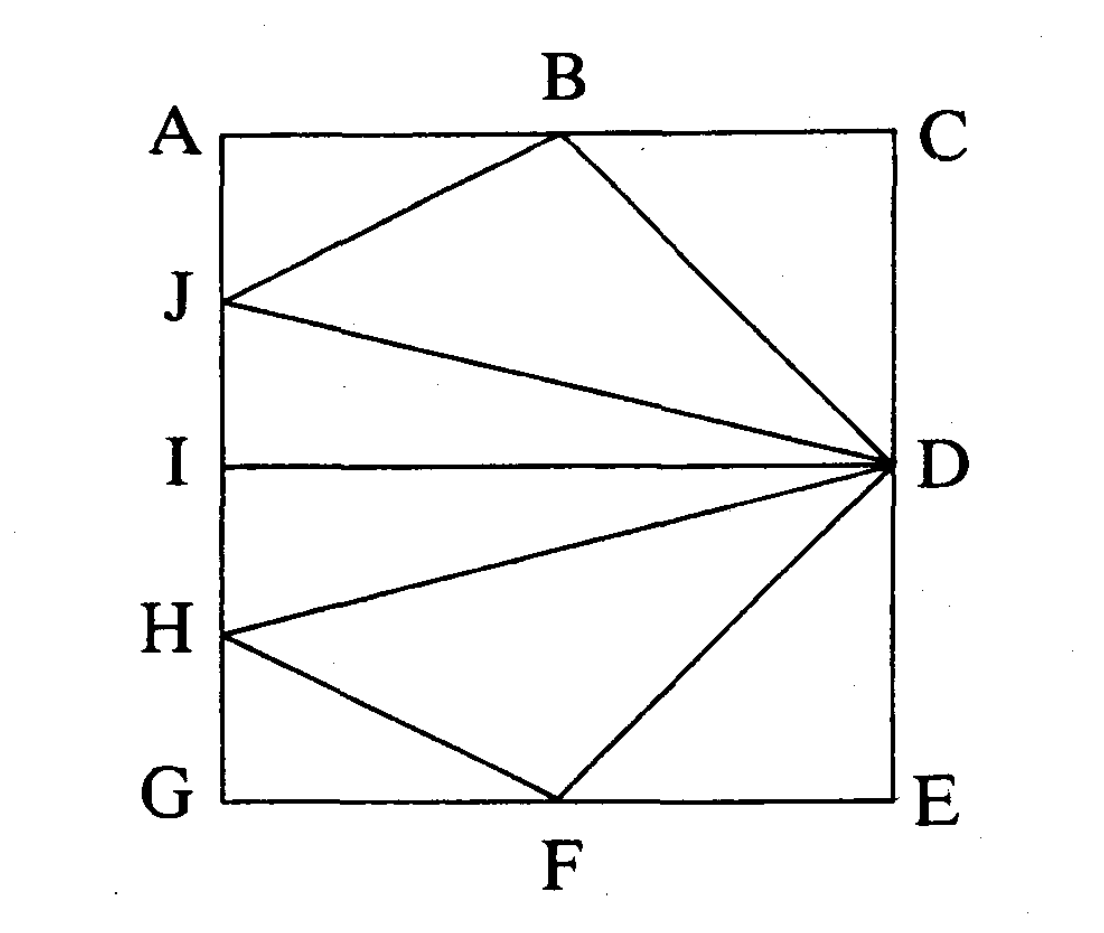
\includegraphics[scale=.15]{introduction/img/rinsma.png}
    \caption{The graph by Rinsma~\cite{Rinsma1987} that is not one-sided.}
    \label{fig:intro:rinsma}
  \end{figure}

\mypar{Overview}
  The rest of this thesis is focused on obtaining these results.
  In order to do this we treat paths and cycles in the remainder of this section. In Section \ref{s:rel} we introduce the notion of regular edge labellings which we use in the rest of the thesis. A regular edge labbeling is a way of coloring and orienting the edges of a graph that corresponds to a rectangular dual of that graph.
  Once we have the preliminaries out of the way we prove Theorem \ref{fix:th:family} in Section \ref{s:fix} and Theorem \ref{th:dsided} in Section \ref{s:algo}. The proof of Theorem \ref{fix:th:family} is by counterexample while the proof of Theorem \ref{th:dsided} is provided by giving a constructive algorithm.


\mypar{Paths and Cycles}
  In the rest of the thesis we frequently need paths and cycles, hence we define them here.

  A path $\P$ is a sequence of vertices such that every two consecutive vertices are connected by an edge. The first and last vertex of the path are its \emph{extreme} vertices while the rest are \emph{internal} vertices of this path. The \emph{length} of a path is the number of edges used to connect the vertices. That, is one less than the number of vertices. In this thesis all paths are \emph{simple}, that is, no vertex occurs twice in the path except possibly the extreme vertices.

  A cycle is a path whose extreme vertices coincide. Because a cycle is a path the start and end vertex are the only vertices that occurs more than once. We call a cycle of length $k$  a \emph{$k$-cycle}. A \emph{triangle} is cycle of length $3$ (i.e. a $3$-cycle). By Jordan's curve theorem a cycle splits the plane into two parts, one bounded and one unbounded. We call the bounded part the \emph{interior} of this cycle and the unbounded part the \emph{exterior} of this cycle.
  Furthermore, the cycle of all vertices bordering the outer face is the \emph{outer cycle}.
  We call a cycle \emph{separating} if there are vertices in both its interior and exterior.
  An \emph{interior edge} of a cycle is then an edge contained in the interior of the cycle.
  An \emph{interior path} is a path connecting two distinct vertices off the cycle and whose edges are interior edges.
